\section{\AP{}Introduction}
\label{sec:intro}

\subsection{\AP{}Graph Databases}

"Graph databases" have gained significant attention due to their ability to efficiently model and manage complex, interconnected data. Unlike traditional relational databases, they model data as entities connected by edges that represent relationships.
This structure facilitates the analysis of highly interconnected data, where the topology of the connections is as crucial as the data itself, making them particularly well-suited for use cases like biology, social networks, banking, recommendation systems, and fraud detection. We refer the reader to \cite{Barcelo2013Querying,Wood2012Query,AnglesEtal2017Foundations} for surveys on the foundations and applications of graph databases.

\todo{}


\subsection{\AP{}Contributions}
% \remi{Please check this subsection. I had to move some paragraphs around ("closed under sublanguages") was defined after its first use.}
Here we solve both the "semantic tree-width $k$ problem" and "one-way semantic tree-width $k$ problem" for every $k$ with one unifying approach.
\begin{theorem}
    \AP\label{thm:decidability-semtw}
    For each $k \geq 1$, the "semantic tree-width $k$ problem" and the "one-way semantic tree-width $k$ problem" are decidable. Moreover, these problems are in "2ExpSpace" and are "ExpSpace"-hard.
	When $k=1$, the problems are in fact "ExpSpace"-complete.
\end{theorem}
In \Cref{sec:maximal-under-approximations} (\Cref{lem:sem-tw-in-twoexp}),
we prove the upper bound for $k\geq 2$, by relying on the so-called ``"Key Lemma"'', which is our main technical result, and is proven in \Cref{sec:treedec,sec:proof-key-lemma}.
The upper bound for the case $k=1$---which was already proven in \cite{BarceloRomeroVardi2016SemanticAcyclicity} for the (two-way) "semantic tree-width $1$ problem"---is shown in \Cref{sec:acyclic-queries} (\Cref{cor:sem-tw-1-pb-exp-c}). The lower bound is shown in \Cref{sec:lowerbound} (\Cref{lemma:lowerbound}).

The "Key Lemma" (\Cref{lemma:bound_size_refinements}) essentially states that
every "UC2RPQ" has a computable ``maximal under approximation'' by a "UC2RPQ" of "tree-width" $k$ and that this approximation is well-behaved with respect to the class of languages used to label the queries under some mild assumptions on it (being ``"closed under sublanguages"''). Let us first
explain this assumption before formalizing the statement above (stated as \Cref{cor:mua-exists-effective}).

For a class $\+L$ of languages, let $\intro*\UCtwoRPQ(\+L)$ denote the class of all "UC2RPQs" whose atoms are all labelled by languages from $\+L$.
\AP For an NFA $\+A$ and two states $q,q'$ thereof, we denote by $\intro*\subaut{\+A}{q}{q'}$ the ""sublanguage"" of $\+A$ recognized  when considering $\set{q}$ as the set of initial states and $\set{q'}$ as the set of final states.
\AP We say that $\+L$ is ""closed under sublanguages"" if
(i) it contains every language of the form $\{a\}$,
where $a \in \A$ is any (positive) letter such that either $a$ or $a^-$ occur in a word of a
language of $\+L$, and (ii) for every language $L \in \+L$ there exists an NFA $\+A_L$ accepting $L$ such that every "sublanguage" $\subaut{\+A_L}{q}{q'}$ distinct from $\emptyset$ and
$\{\varepsilon\}$ belongs to $\+L$.

To the best of our knowledge,
all classes of regular expressions that have been considered in the realm of regular path queries (see, "eg", \cite[\S1]{FigueiraEtal2020Containment}) are "closed under sublanguages". In particular, this is
the case for the class $\bigl\{ \{a_1+\hdots+a_n\} \mid a_1,\hdots,a_n
\in \A \bigr\} \cup \bigl\{ a^* \mid a \in \A \bigr\}$, which will be our focus of study in \Cref{sec:sre}. Moreover, even if some class $\+L$
is not "closed under sublanguages", such as $\{(aa)^*\}$,
then it is contained in a minimal class "closed under sublanguages"---$\{a, a(aa)^*, (aa)^*\}$ in 
this example.

We can now state the main implication of the "Key Lemma" (whose formal statement requires some extra definitions).
\begin{restatable*}[Existence of the "maximal under-approximation"]{cor}{muaexistseffective}
    \AP\label{cor:mua-exists-effective}
    % Fix $k > 1$ and a class $\+L$ of regular languages closed under "sublanguages". Then, every $\UCtwoRPQ(\+L)$ query has a 
    % "maximal under-approximation" by infinitary unions of $\Tw$ queries that can be effectively computed as a $\UCtwoRPQ(\+L)$ query in "ExpSpace".
    For each $k \geq 2$, for each class $\+L$ "closed under sublanguages",
    and for each query $\Gamma \in \UCtwoRPQ(\+L)$,
    there exists $\Gamma' \in \UCtwoRPQ(\+L)$ of "tree-width" at most $k$ 
    such that
    $\Gamma' \contained \Gamma$, and for every $\Delta \in \UCtwoRPQ$, if $\Delta$ has
    "tree-width" at most $k$ and $\Delta \contained \Gamma$, then $\Delta \contained \Gamma'$.
    Moreover, $\Gamma'$ is computable from $\Gamma$ in "ExpSpace".
\end{restatable*}

As a consequence of \Cref{cor:mua-exists-effective,prop:crpq-bound-tree-width-upper-bound}, we have that queries of bounded "semantic tree-width" have tractable evaluation.
\begin{restatable*}[FPT evaluation for bounded "semantic tree-width"]{cor}{fptEvalBoundedSemTreeWidth}
	\AP\label{coro:fpt-eval-bounded-semtreewidth}
	For each $k\geq 1$, the "evaluation problem" for "C2RPQs" of "semantic tree-width"
	at most $k$ is fixed-parameter tractable---"FPT"---when parametrized in the size of
	the query. More precisely on input $\langle \Gamma, G \rangle$,
	the algorithm runs in time
	$\+O(f(\size{\Gamma})\cdot |G|^{k+1} \cdot \log{|G|})$ on a Turing machine, where $f$ is a doubly-exponential function---or $\+O(f(\size{\Gamma})\cdot |G|^{k+1})$ under a RAM model.
\end{restatable*}
Note that \cite[Theorem~22]{FeierGogaczMurlak24Treewidth} shows that the statement above can be improved to have a single-exponential function $f$.

% Essentially, this means that to minimize the "semantic tree-width" of a query, we do not need to ``create'' new languages.
% 138/139 and 153/154: It took me a while to see why this does not follow from the definition. It 
% would have helped me, if there was an informal pointer that semantic acyclicity always refers 
% to 2-way CRPQs (for understanding this I also looked at Barcelo/Romero/Vardi,
% there it also took me a moment).
% In other words, if a query
% can be defined with labels in $\+L$, and if this query is equivalent to a  
% query of small tree-width, then it is also equivalent to a query of small tree-width
% with labels in $\+L$.
% In particular, for any $k>1$, a "CRPQ" is equivalent to a "UC2RPQ" of "tree-width" at most $k$ if{f} it is e equivalent to "UCRPQ" of "tree-width" at most $k$, which is not true for $k=1$ ("cf" \Cref{rk:closure-under-sublanguages-k1}, also \cite[Proposition 6.4]{BarceloRomeroVardi2016SemanticAcyclicity}).

Moreover, we also show that for any class $\+L$ of regular languages "closed under sublanguages", if $\Gamma \in \UCtwoRPQ(\+L)$ has "semantic tree-width" $k > 1$,
then $\Gamma$ is equivalent to a $\UCtwoRPQ(\+L)$ of "tree-width" at most $k$.
Analogous characterizations hold for $k=1$ and/or "path-width", see \Cref{coro:charact-semantic-treewidth-1,coro:charact-semantic-pathwidth-k}.

\begin{restatable*}{theorem}{closureundersublanguages}
    \AP\label{thm:closure-under-sublanguages}
    \AP Assume that $\+L$ is "closed under sublanguages". 
    For any $k > 1$ and any query $\Gamma \in \UCtwoRPQ(\+L)$, the following are equivalent:
    \begin{enumerate}
        \itemAP[\introinrestatable{\itemClosureInfCQ}] $\Gamma$ is "equivalent" to an "infinitary union" of "conjunctive queries"
            of "tree-width" at most $k$; \label{thm:closure-under-sublanguages:1}
        \itemAP[\introinrestatable{\itemClosureUCRPQ}] $\Gamma$ has "semantic tree-width" at most $k$; \label{thm:closure-under-sublanguages:2}
        \itemAP[\introinrestatable{\itemClosureUCRPQSimple}] $\Gamma$ is "equivalent" to a $\UCtwoRPQ(\+L)$ of "tree-width" at most $k$. \label{thm:closure-under-sublanguages:3}
    \end{enumerate}
\end{restatable*}

The implications $\itemClosureUCRPQSimple \Rightarrow \itemClosureUCRPQ \Rightarrow \itemClosureInfCQ$ immediately follow
from the definition of the "semantic tree-width".
On the other hand, the
implications $\itemClosureInfCQ \Rightarrow \itemClosureUCRPQ$ and $\itemClosureUCRPQ \Rightarrow \itemClosureUCRPQSimple$ are surprising,
since they are both trivially false when $k=1$. We defer the proof of this last claim
to \Cref{rk:closure-under-sublanguages-k1} as we first need a few tools to manipulate "CRPQs".

% The proof of our "key lemma" spans over
% \Cref{sec:approximations,sec:treedec,sec:proof-approximations}:
% in \Cref{sec:approximations}, we introduce necessary notions to formally state it,
% and deduce \Cref{thm:decidability-semtw,thm:closure-under-sublanguages} from it;
% in \Cref{sec:treedec} we introduce the central notion of "tagged tree decompositions"
% of "C2RPQs homomorphisms", and building on it, we finally describe the
% constructions used to prove the "Key Lemma" in \Cref{sec:proof-approximations}.

The previous theorem, together with the high complexity of "semantic tree-width $k$ problem",
motivates us to focus on the case of "CRPQs" using some "simple regular expressions" ("SRE") in \Cref{sec:sre}, where we show that the complexity of this problem is much lower.
% coincides with the complexity of the "containment problem" over this class of "CRPQs" \cite[Corollary~5.2]{FigueiraEtal2020Containment}:

\begin{restatable*}{theorem}{thmSemTwSREpitwo}
    \AP\label{thm:semtw-sre-pitwo}
    For $k\geq 2$, the "semantic tree-width $k$ problem" for {\UCRPQSRE} is in "PiP2".
\end{restatable*}

We then study the problem of $k=1$: at first glance, our proof for $k\geq 2$ of
\Cref{thm:decidability-semtw} does not capture this case, for a technical---yet crucial---reason. In
\Cref{sec:acyclic-queries}, we explain how to adapt our proof to capture it: 
and show the decidability the "semantic tree-width 1 problem"---which was already studied by 
Barceló, Romero and Vardi \cite{BarceloRomeroVardi2016SemanticAcyclicity}---and of the "one-way semantic tree-width 1 problem". 

Building on the same idea, we show in \Cref{sec:semantic-path-width} that our results extend to "path-width".
\begin{restatable*}{theorem}{decidabilitySemPw}
    \AP\label{thm:decidability-sempw}
    For each $k \geq 1$,
    the "semantic path-width $k$ problems" are decidable. Moreover, they lie in "2ExpSpace"
    and are "ExpSpace"-hard. Moreover, if $k=1$, these problems are in fact "ExpSpace"-complete.
\end{restatable*}
In turn, this leads to an evaluation algorithm with a remarkably low complexity.
\begin{restatable*}{theorem}{paraNLEvalBoundedSemPathWidth}
	\AP\label{thm:evaluation-bounded-pathwidth}
	For each $k \geq 1$, the "evaluation problem", restricted to "UC2RPQs" of
	"semantic path-width" at most $k$ is in "para-NL" when parametrized in the size of the query.
	More precisely, the problem, on input $\langle \Gamma, G \rangle$, can be solved in
	non-deterministic space $f(|\Gamma|) + \log(|G|)$, where $f$ is a single exponential
	function.
\end{restatable*}

\begin{figure}
	\centering
	\subfloat[Semantic classes of "C2RPQs" related to "tree-width".]{
		\AP\label{fig:taxonomy-semantic-tw}
		% \scalebox{1.125}{
		\begin{tikzpicture}
			\node at (0,0) {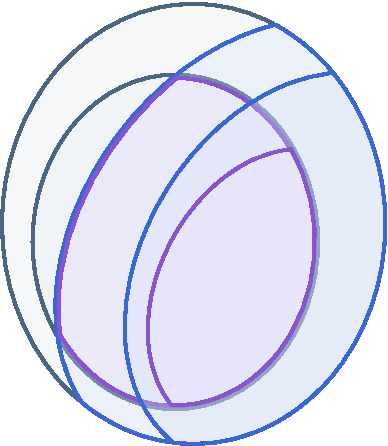
\includegraphics[scale=.8]{taxonomy-semantic-tw.pdf}};
			% \draw[line width=1.5pt] (0,-4) -- (0,4);
			% \draw[line width=1.5pt] (-3,0) -- (3,0);
			% \draw[line width=.5pt] (1,-4) -- (1,4);
			% \draw[line width=.5pt] (-3,1) -- (3,1);
			% \draw[line width=.5pt] (-1,-4) -- (-1,4);
			% \draw[line width=.5pt] (-3,-1) -- (3,-1);
			\node[font=\tiny, align=center] at (.6,-.7)
				{\kl[one-way semantic tree-width]{\color{cPurple}1way sem.}\\ \kl[one-way semantic tree-width]{\color{cPurple}tw 1}};
			\node[font=\tiny, align=center] at (-1,.3)
				{\kl[one-way semantic tree-width]{\color{cPurple}1way}\\ \kl[one-way semantic tree-width]{\color{cPurple}sem.}\\ \kl[one-way semantic tree-width]{\color{cPurple}tw $k$}};
			\node[font=\tiny, align=center] at (1.9,.9)
				{\kl[semantic tree-width]{\color{cBlue}sem.}\\ \kl[semantic tree-width]{\color{cBlue}tw 1}};
			\node[font=\tiny, align=center] at (1,2.2)
				{\kl[semantic tree-width]{\color{cBlue}sem.}\\ \kl[semantic tree-width]{\color{cBlue}tw $k$}};
			\node[font=\tiny] at (-1.6,.8) {\kl[CRPQ]{\rotatebox{60}{\color{cDarkGrey}CRPQs}}};
			\node[font=\tiny] at (-.5,2.4) {\kl[C2RPQ]{\color{cDarkGrey}C2RPQs}};
		\end{tikzpicture}
		% }
	}
	\hfill
	\subfloat[Semantic classes of "C2RPQs" related to "path-width".]{
		\AP\label{fig:taxonomy-semantic-pw}		
		\centering 
		% \scalebox{1.125}{
		\begin{tikzpicture}
			\node at (0,0) {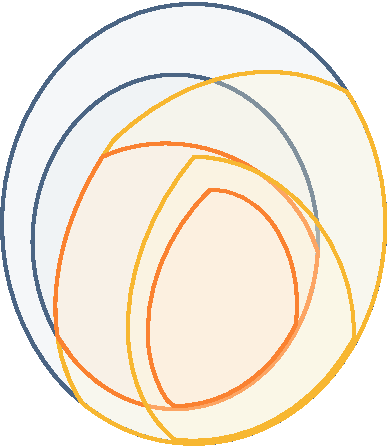
\includegraphics[scale=.8]{taxonomy-semantic-pw.pdf}};
			% \draw[line width=1.5pt] (0,-4) -- (0,4);
			% \draw[line width=1.5pt] (-3,0) -- (3,0);
			% \draw[line width=.5pt] (1,-4) -- (1,4);
			% \draw[line width=.5pt] (-3,1) -- (3,1);
			% \draw[line width=.5pt] (-1,-4) -- (-1,4);
			% \draw[line width=.5pt] (-3,-1) -- (3,-1);
			\node[font=\tiny, align=center] at (.4,-1)
				{\kl[one-way semantic path-width]{\color{cOrange}1way sem.}\\ \kl[one-way semantic path-width]{\color{cOrange}pw 1}};
			\node[font=\tiny, align=center] at (-1.1,0)
				{\kl[one-way semantic path-width]{\color{cOrange}1way}\\ \kl[one-way semantic path-width]{\color{cOrange}sem.}\\ \kl[one-way semantic path-width]{\color{cOrange}pw $k$}};
			\node[font=\tiny] at (1,-2.35) {\kl[semantic path-width]{\rotatebox{33}{\color{cYellow}sem. pw 1}}};
			\node[font=\tiny, align=center] at (1.9,.9)
				{\kl[semantic path-width]{\color{cYellow}sem.}\\ \kl[semantic path-width]{\color{cYellow}pw $k$}};
			\node[font=\tiny] at (-1.6,.8) {\kl[CRPQ]{\rotatebox{60}{\color{cDarkGrey}CRPQs}}};
			\node[font=\tiny] at (-.5,2.4) {\kl[C2RPQ]{\color{cDarkGrey}C2RPQs}};
		\end{tikzpicture}
		% }
	}
	\caption{
		\AP\label{fig:taxonomy-semantic}
		Clickable taxonomy of semantic classes studied in this chapter, where $k \geq 2$.
		(To be compared with \Cref{fig:taxonomy-syntactic}.)
	}
\end{figure}
Interestingly, the proof for "tree-width" 1 and "path-width" $k$ ($k \geq 1$)
can be derived from the proof from "tree-width" $k\geq 2$ but necessitates an
additional technical trick which yields different closure properties (or lack thereof).
We show that a "UCRPQ" has "semantic tree-width" at most $k$ if, and only if, it
has "one-way semantic tree-width" at most $k$ whenever $k \geq 2$
(\Cref{coro:collapse-twoway-oneway-semtw}). In other words, if the original query does not
use "two-way navigation", then considering "UC2RPQs" does not help to further minimize the "tree-width". Interestingly, this is false for $k=1$ ("cf" \Cref{rk:closure-under-sublanguages-k1},
also \cite[Proposition 6.4]{BarceloRomeroVardi2016SemanticAcyclicity}) and for "path-width", no matter the value of $k\geq 1$ (see \Cref{rk:path-width:oneway-vs-twoway}). Overall, this leads to
the landscape depicted in \Cref{fig:taxonomy-semantic}.

Finally, we conclude in \Cref{sec:discussion}.
We provide a \emph{partial} characterization \emph{à la} Grohe of classes of "UC2RPQs" which admit a tractable evaluation in \Cref{sec:charact-tractability}.
\begin{restatable*}{theorem}{thmtractabilityfinred}
    \AP\label{thm:tractability-finred}
    Assuming $"W[1]" \neq $ "FPT", for any recursively enumerable class $\+C$ of "finitely-redundant" Boolean "UC2RPQs", the "evaluation problem" for $\+C$ is "FPT" if, and only if, $\+C$ has bounded "semantic tree-width".
\end{restatable*}
We also discuss open questions, ranging from complexity
questions (\Cref{sec:discussion-complexity}) to extensions of our results to bigger classes
or larger settings (\Cref{sec:discussion-larger-classes,sec:discussion-different-notions}).

% \subsection{\AP{}Conference Paper}
% \label{sec:conf-paper-diff}
% The current article is based on the conference paper \cite{FigueiraMorvan2023SemanticTreeWidthICDT}. The main results for "tree-width" $k>1$ are essentially the same---though with improved explanations and figures, and we fixed some minor bugs in the proof of the "Key Lemma". Here we also show how to extend our techniques to tackle the "semantic tree-width $1$ problem" (\Cref{sec:acyclic-queries}) and we introduce and study the "semantic path-width $k$ problems" (\Cref{sec:semantic-path-width}). Our very partial lift of Grohe's characterization of "FPT" classes of queries (\Cref{thm:tractability-finred}) is also new.